\section{Ход работы}
\subsection{Измерения}
1. Основные величины, которые были измерены самыми первыми:
\begin{itemize}
    \item диаметр малого шкива $d_1 = (18,9 \pm 0,1)$ мм
    \item диаметр большого шкива $d_2 = \left(35,9 \pm 0,1\right)$ мм
    \item для 2 и 3 расстояние между грузами 225 мм
\end{itemize}
\begin{center}
\begin{tabular}{|c|c|c|c|c|}
    \hline
    Номер груза & Масса груза, г & Высота груза, мм & Диаметр груза, мм \\
    \hline
    4.1 & 155,5 & 25,0 & 32,9 \\
    \hline
    4.2 & 148,9 & 25,1 & 32,9 \\
    \hline
    4.3 & 151,9 & 25,0 & 32,9 \\
    \hline
    4.4 & 150,1 & 25,0 & 33,0 \\
    \hline
\end{tabular}
\end{center}

2. Теперь измерим показатели $k$ и $\beta_0$ для маятника без грузов:

\begin{center}
\begin{tabular}{|c|c|c|c|}
    \hline
    Направление & $k$, 1/с & $\beta_0$, 1/с$^2$ & $m_\text{н}$, г \\
    \hline
    Вверх & $-0,03424 \pm 0,0018$ & $3,147 \pm 0,0057$ & 110,1 \\
    \hline
    Вниз &$-0,0419 \pm 0,004$ & $3,014 \pm 0,0077$ & 110,1 \\
    \hline
    Вверх &$-0,0661 \pm 0,015$ & $2,184 \pm 0,028$ & 72,1 \\
    \hline
    Вниз &$-0,04039 \pm 0,0025$ & $1,996 \pm 0,0062$ & 72,1 \\
    \hline
    Вверх &$-0,05968 \pm -0,013$ & $1,776 \pm 0,023$ & 60 \\
    \hline
    Вниз &$-0,03976 \pm 0,0045$ & $1,664 \pm 0,0095$ & 60 \\
    \hline
\end{tabular}
\end{center}



3. Далее рассмотрим вращение маятника с грузами при закрчивании нити на большой шкив:
\begin{center}
\begin{tabular}{|c|c|c|c|}
    \hline
    Направление & $k$, 1/с & $\beta_0$, 1/с$^2$ & $m_\text{н}$, г \\
    \hline
    Вверх & $-0,01922 \pm 0,004$ & $1,361 \pm 0,0086$ & 110,1 \\
    \hline
    Вниз &$-0,01643 \pm 0,0011$ & $1,324 \pm 0,0028$ & 110,1 \\
    \hline
    Вверх &$-0,02582 \pm 0,0053$ & $1,398 \pm 0,0091$ & 110,1 \\
    \hline
    Вниз &$-0,01409 \pm 0,0019$ & $1,337 \pm 0,0046$ & 110,1 \\
    \hline
    Вверх &$-0,01509 \pm 0,00099$ & $1,332 \pm 0,00096$ & 110,1 \\
    \hline
    Вниз &$-0,01714 \pm 0,0015$ & $1,317 \pm 0,0029$ & 110,1 \\
    \hline
    Вверх &$-0,01322 \pm 0,0022$ & $0,8557 \pm 0,0021$ & 72,1 \\
    \hline
    Вниз &$-0,01645 \pm 0,0011$ & $0,8592 \pm 0,0012$ & 72,1 \\
    \hline
    Вверх &$-0,01268 \pm 0,0012$ & $0,8537 \pm 0,001$ & 72,1 \\
    \hline
    Вниз &$-0,01457 \pm 0,0013$ & $0,8739 \pm 0,0019$ & 72,1 \\
    \hline
    Вверх &$-0,01077 \pm 0,0012$ & $0,8401 \pm 0,0012$ & 72,1 \\
    \hline
    Вниз &$-0,01464 \pm 0,001$ & $0,8747 \pm 0,0016$ & 72,1 \\
    \hline
    Вверх &$-0,01157 \pm 0,0021$ & $0,697 \pm 0,0019$ & 60 \\
    \hline
    Вниз &$-0,01437 \pm 0,0012$ & $0,7255 \pm 0,001$ & 60 \\
    \hline
    Вверх &$-0,01787 \pm 0,0057$ & $0,7172 \pm 0,0075$ & 60 \\
    \hline
    Вниз &$-0,01402 \pm 0,0017$ & $0,7273 \pm 0,0036$ & 60 \\
    \hline
    Вверх &$-0,01531 \pm 0,0013$ & $0,7414 \pm 0,0011$ & 60 \\
    \hline
    Вниз &$-0,01351 \pm 0,0015$ & $0,7641 \pm 0,0027$ & 60 \\
    \hline
\end{tabular}
\end{center}

4. Далее рассмотрим вращение маятника с грузами при закрчивании нити на малый шкив:
\begin{center}
\begin{tabular}{|c|c|c|c|}
    \hline
    Направление & $k$, 1/с & $\beta_0$, 1/с$^2$ & $m_\text{н}$, г \\
    \hline
    Вверх & $-0,003826 \pm 0,0014$ & $0,3444 \pm 0,00082$ & 60 \\
    \hline
    Вниз &$-0,01046 \pm 0,00087$ & $0,4352 \pm 0,0012$ & 60 \\
    \hline
    Вверх &$-0,005627 \pm 0,0026$ & $0,3494 \pm 0,001$ & 60 \\
    \hline
    Вниз &$-0,01134 \pm 0,0016$ & $0,4279 \pm 0,0023$ & 60 \\
    \hline

\end{tabular}
\end{center}

5. Далее рассмотрим вращение маятника с грузами при закрчивании нити на большой шкив, но с другим расстоянием между грузами (312 мм):

\begin{center}
\begin{tabular}{|c|c|c|c|}
    \hline
    Направление & $k$, 1/с & $\beta_0$, 1/с$^2$ & $m_\text{н}$, г \\
    \hline
    Вверх & $-0,008358 \pm 0,0017$ & $0,5206 \pm 0,0017$ & 60 \\
    \hline
    Вниз &$-0,001135 \pm 0,0012$ & $0,558 \pm 0,0021$ & 60 \\
    \hline
    Вверх &$-0,008094 \pm 0,0013$ & $0,526 \pm 0,0012$ & 60 \\
    \hline
    Вниз &$-0,01042 \pm 0,0015$ & $0,5627 \pm 0,0013$ & 60 \\
    \hline
    Вверх &$-0,001018 \pm 0,0023$ & $0,5309 \pm 0,0015$ & 60 \\
    \hline
    Вниз &$-0,01011 \pm 0,00065$ & $0,5639 \pm 0,00059$ & 60 \\
    \hline

\end{tabular}
\end{center}

6. Далее рассмотрим вращение маятника с грузами при закрчивании нити на большой шкив, но с другим расстоянием между грузами (382 и 375 мм):

\begin{center}
\begin{tabular}{|c|c|c|c|}
    \hline
    Направление & $k$, 1/с & $\beta_0$, 1/с$^2$ & $m_\text{н}$, г \\
    \hline
    Вверх & $-0,008433 \pm 0,00037$ & $0,3982 \pm 0,00018$ & 60 \\
    \hline
    Вниз &$-0,006391 \pm 0,00093$ & $0,4259 \pm 0,00079$ & 60 \\
    \hline

\end{tabular}
\end{center}

\subsection{Обработка}

7. Из (3) можно посчитать момент инерции для маятника без грузов:
\begin{equation*}
    I_0 \approx \frac{m_\text{н}gr}{\beta_0} = (62 \pm 1)\cdot 10^{-4} \text{ кг} \cdot \text{м}^2
\end{equation*}

8. Посчитаем $M_\text{н}$ для большого шкива:
\[M (m = 110\text{ г})  = (193 \pm 1) \cdot 10^{-4} \text{ Н} \cdot \text{м}^2,\]
\[M (m = 72\text{ г})  = (127 \pm 1) \cdot 10^{-4} \text{ Н} \cdot \text{м}^2,\]
\[M (m = 60\text{ г})  = (106 \pm 1) \cdot 10^{-4} \text{ Н} \cdot \text{м}^2.\]

9. Для малого шкива:
\[M (m = 60\text{ г})  = (56 \pm 1) \cdot 10^{-4} \text{ Н} \cdot \text{м}^2.\]

10. Аналогичные иземерения для изменения расстояния между грузами:
\[M (\rho = 312 \text{ мм})  = (106 \pm 1) \cdot 10^{-4} \text{ Н} \cdot \text{м}^2,\]
\[M (\rho = 379 \text{ мм})  = (106 \pm 1) \cdot 10^{-4} \text{ Н} \cdot \text{м}^2.\]
Заметим, что отклонений от значений в пункте 8 нет.

11. Построим зависимость $M(\beta_0)$ для значений из 8 и 9:
\begin{figure}[H]
    \centering
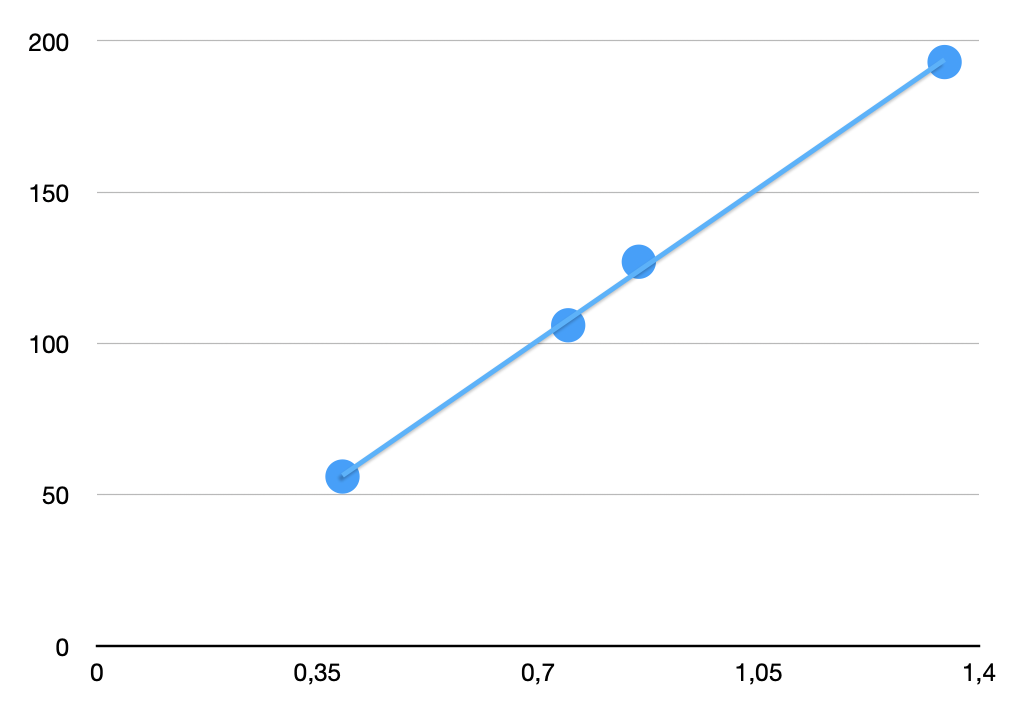
\includegraphics[width=0.75\linewidth,center]{p2.png}
    \label{fig:my_label}
\end{figure}
Получилось уравнение $M (\beta_0) = (143,8 \cdot \beta_0 - 0,4) \cdot 10^{-4} \text{ Н} \cdot \text{м}^2 \approx const$, где $\beta_0$ в 1/с$^2$, что
говорит, что мы идём в правильном направлении, так как это уравнение
приблизительно соответствует уравнению вращательного движения.

Добавка $M_\text{тр} = 4 \cdot 10^{-5} \text{ Н} \cdot \text{м}^2$ объясняется наличием силы трения.

Из этого уравнения $I = (143,8 \pm 2,5) \cdot 10^{-4} \text{ кг} \cdot \text{м}^2$.

12. Посчитаем суммарный момент инерции по (5) и высчитаем из него $I_0$:

\[I_0 = (67 \pm 3) \cdot 10^{-4} \text{ кг} \cdot \text{м}^2\]

13. Получилась зависимость $\beta_0(\rho)$. По этой зависимости посчитаем
$I = \frac{M}{\beta_0}$ и $I_0 = I - \sum_{i = 1}^{4}\left(I_i + m_i R_i^2\right)$:

на данном этапе была слишком большая погрешность (относительная > 50\%), что говорит о том, что при измерениях допущены ошибки.
